% chapter 11 b - jean
\documentclass[../main.tex]{subfiles}

\newcommand\crit[1]{V\if\relax\detokenize{#1}\relax\else(#1)\fi}
\newcommand\postcrit[1]{P\if\relax\detokenize{#1}\relax\else(#1)\fi}
\newcommand\postcl[1]{\cl{P}\if\relax\detokenize{#1}\relax\else(#1)\fi}

\newcommand\dist[3][]{\operatorname{dist}_{#1}({#2}, {#3})}
%\newcommand\norm[1]{\left\lVert#1\right\rVert}
\newcommand\deriv[2]{D {#2}_{#1}}
\begin{document}

\subsection{The Postcritical Closure}

\note{\textbf{this draft of the final section yet contains much content that is incomplete and incorrect. It is expected that these issues will be brought up for discussion during the Tuesday meeting.}}

In the previous sections, we've shown that every attracting fixed point attracts a critical point, and that every parabolic fixed point contains a critical point in each of its basins. For an irrationally indifferent fixed point, there are again relations, albeit less direct, between the dynamics and the set of critical points.

\begin{dfn}
The \emph{postcritical set} $\postcrit{} = \postcrit{f}$ of $f$ is the union of the strict forward orbits of its critical points:
\[
    \postcrit{f} = \bigcup\limits_{k > 0} f^k(\crit{f})
\]
Where $\crit{f} = \{ z \in \C \mid f'(z) = 0 \}$. The \emph{postcritical closure} \postcl{f} is the topological closure of $\postcrit{f}$.
\end{dfn}

\note{the notation is possibly confusing. Since we almost never refer to $\postcrit{f}$, perhaps it would make sense to just reserve $P$ for the postcritical closure, as is the convention followed in several other sources.}

Equivalently, $\postcl{f}$ is the minimal closed set which contains all critical values of $f^n$ for every $n > 0$. The main result of this section is that the postcritical closure contains every Cremer point and the boundary of every Siegel disc.

We shall frequently make use of the assumption that the complement $Q = \hat{\C} \setminus \postcl{}$ of the postcritical closure is hyperbolic, which is true if and only if $\postcl{}$ contains at least three points. The following lemma takes care of the exceptional case:

\begin{lem}\label{lem:exceptional-Pf}
If $\postcl{f}$ contains fewer than three points, then $f$ is conjugate to the $n$-th power map $z \mapsto z^n$.
\end{lem}
\begin{proof}
In this case $Q$ is the twice punctured sphere. Since $Q_1 = f\inv(Q)$ contains no critical points of $f$, the restriction $f : Q_1 \to Q$ is a covering map. Since $Q$ is Euclidean, the covering space $Q_1$ is either $\C$ or $\C\setminus\{0\}$; $Q_1$ cannot be conformally isomorphic to $\C$ since $Q$ is not isomorphic to $\C$ and any proper subset of $Q$ is hyperbolic. Thus $Q_1 = Q$. $Q$ has as its fundamental group $\Z$, whose conjugacy classes of subgroups are the subgroups generated by each element of $\Z$. By the correspondence to isomorphism classes of covering maps we conclude that $Q_1$ must map onto $Q$ by a covering map isomorphic to $z \mapsto z^n$.
\end{proof}
\note{can we conclude $Q$ is the twice punctured sphere without Riemann-Hurwitcz?}
\note{the argument shows (we hope) that $Q_1 \to Q$ is \emph{topologically} conjugate to $z \mapsto z^n$. How do we arrive at the stronger conclusion that this conjugation is conformal?}

Thus the dynamics of a map on $\hat{\C}$ whose postcritical closure contains no more than two points are well understood as a special case. In all other cases we have that $Q$ is hyperbolic, and we have available to us the \emph{Poincaré metric}.

\subsubsection{The Poincaré metric}

We begin with the fact that there is a unique, up to a positive constant multiple, Riemannian metric on $\D$ that is invariant under every conformal automorphism of $\D$.

\note{trying to get away from having to introduce additional objects, but shaky about saying the words \emph{Riemannian metric} without even having defined the tangent space. \textbf{to do:} seek advice on structuring this exposition.}

If we in addition impose the condition that the \emph{Gaussian curvature} $K$ is equal to $-1$, then there is exactly one such metric:

\begin{exl}[unit disc]
The Poincaré metric on $\D$ is given by
\[
ds = \frac{2\abs{dz}}{1-\abs{z}^2}
\]
\end{exl}

By uniformisation, every hyperbolic Riemann surface $S$ has the unit disc $\D$ as its universal cover, and is conformally isomorphic to some quotient of $\D$ by a group of all free and properly discontinuous conformal automorphisms of $\D$. Since the Poincaré metric on $\D$ is invariant under conformal automorphisms, by requiring that the projection $\D \to S$ be a local isometry, we recover a well-defined metric on $S$, which we call the \emph{Poincaré metric} on $S$.

\note{Milnor 2.1. Trying to figure out which details can be omitted for the exposition to still sort of make sense.}

\begin{exl}[punctured disc]
The Poincaré metric on $\D\setminus \{0\}$ is given by
\[
ds = \frac{\abs{dz}}{\abs{z} \log(1/\abs{z})}
\]
which can be seen by observing the Poincaré metric on the unit disc as it is taken through a conformal isomorphism to the half plane then to the punctured disc.
\end{exl}

Equipped with a metric, it now makes sense to speak of the \emph{distance} between two points on a hyperbolic Riemann surface $S$, by defining $\dist{z_1}{z_2}$ to be the infimum over all piecewise-smooth paths $\gamma : [0, 1] \to S$ joining $z_1$ and $z_2$ of the \emph{length} $\int_\gamma ds$ of $\gamma$.

\begin{thm}[Schwarz-Pick]\label{thm:2.11}
Let $S, T$ be hyperbolic Riemann surfaces and $f: S \to T$ be holomorphic. Then $f$ is (with respect to the Riemannian metrics of $S$ and $T$) a local isometry if and only if it is a covering map, a \emph{global} isometry if and only if the covering is trivial, and strictly decreases all nonzero distances in all other cases. More explicitly, exactly one of the following three cases is true:
\begin{itemize}
    \item \emph{isometry.} $f$ is a conformal isomorphism and an isometry with respect to the Poincaré metrics on $S$ and $T$.
    \item \emph{covering.} $f$ is a nontrivial covering map. In this case $f$ is a local isometry, but not a global isometry. Furthermore we have
    \[
    \dist[T]{f(z_1)}{f(z_2)} \le \dist[S]{z_1}{z_2}
    \]
    for all $z_1, z_2 \in S$.
    \item \emph{contraction.} $f$ strictly decreases all non-zero distances. Furthermore, for compact $K \subseteq S$, there exists constant $c < 1$ such that
    \[
    \dist[T]{f(z_1)}{f(z_2)} \le c\dist[S]{z_1}{z_2}
    \]
    for all $z_1, z_2 \in K$, and every smooth path $\gamma : [0, 1] \to S$ in $K$ with arclength $\ell$ maps to a path $f \circ \gamma$ with arclength no greater than $c\ell$ in $T$.
\end{itemize}
\end{thm}

In particular, if $\dist[T]{f(z_1)}{f(z_2)} \le c \dist[S]{z_1}{z_2}$ for all $z_1, z_2$ in some neighbourhood of $z_0$, then equivalently $\norm{\deriv{z_0}{f}} \le c$, with the norm of the derivative $\deriv{z}{f}: T_{z}S \mapsto T_{f(z)}T$ evaluated with respect to the Poincaré metric on $S$ and $T$.

\note{this remark should probably be a longer, better-justified exposition; objects like $K$ or $\deriv{z}{f}$ doesn't make a lot of sense under this abridged treatment of the metric.}

\subsubsection{Expansion on the complement of the postcritical closure}

In this section we work towards a result which relates  but by way of following the Poincaré metric on the complement of the postcritical closure: notably we show that $f$ is \emph{expanding} at every point in the Julia set of $f$ whose forward orbit does not meet $\postcl{f}$.

We begin with the following bound: intuitively it states that the norm of the the derivative $\deriv{z}{\iota}$ of an inclusion map $\iota: S \to T$ is small if $z$ is close to the boundary of $S$ in $T$.

\begin{lem}
let $\iota : S \to T$ be the inclusion of one hyperbolic Riemann surface into another. Then $\norm{\deriv{z}{\iota}}$ is bounded within a constant multiple of $\abs{s \log s}$ as $s \tendsto 0$, in which $s = \dist[V]{z}{T \setminus S}$.
\end{lem}
\begin{proof}(compose with conformal isometry to reduce to the case $\D\setminus\{0\} \to \D$ and use expressions for respective Poincaré metrics)\end{proof}

Before we continue, let us extrapolate some notation: we define the iterated preimages $P_n$ of $\postcl{}$:
\[
    P_n = f^{-n}(\postcl{})
\]

and for their complements we write $Q_n = \hat{\C} \setminus P_n$. Note that the $P_n$ are compact and forward invariant:
\[
\postcl{} = P_0 \subseteq P_1 \subseteq P_2 \subseteq
\cdots \subseteq P_n \subseteq \cdots
\]
and correspondingly the $Q_n$ are open and backward invariant:
\[
Q = Q_0 \supseteq Q_1 \supseteq Q_2 \supseteq
\cdots \supseteq Q_n \supseteq \cdots
\]

We note also that since $Q_n$ contains no critical points of $f^n$, the restrictions $f^n : Q_n \to Q$ are covering maps.

\begin{lem}\label{lem:julia-in-cl-union}
Let $f : \hat{\C} \to \hat{\C}$ be holomorphic and suppose $\abs{\postcl{f}} \ge 3$. Then the Julia set is contained in the closure of $\bigcup_{n \ge 0} P_n$. In particular, for every $z$ in the Julia set,
\[
\dist[Q]{z}{P_n} \tendsto 0 \quad\text{as}\quad n \tendsto \infty
\]
\end{lem}
\begin{proof} (Montel + Hausdorff distance) \end{proof}

\begin{lem}\label{lem:deriv-bound}
Let $f : \hat{\C} \to \hat{\C}$ be holomorphic and suppose $\abs{\postcl{f}} \ge 3$. For all $z$ such that $f(z) \notin \postcl{f}$, we have
\[
\norm{\deriv{z}{f}} \ge 1
\]
with respect to the Poincaré metric on $Q$.
\end{lem}
\begin{proof}
Equivalently we show that $f$ is contracting with respect to the Poincaré metric on $Q$. Take any $z_1, z_2 \in Q_1$, i.e. for any $z_1, z_2$ whose images fall not in $\postcl{}$.
Recall that $f : Q_1 \to Q$ is a covering map hence a local isometry by Pick's theorem (\ref{thm:2.11}). The inclusion map $\iota : Q1 \to Q$ is contracting, again by \ref{thm:2.11}. Together
\[
\dist[Q]{z_1}{z_2} \ge \dist[Q_1]{z_1}{z_2} = \dist[Q]{f(z_1)}{f(z_2)}
\]
which gives the desired result.
\end{proof}

The next lemma proceeds in a similar manner:

\begin{lem}
Let $f : \hat{\C} \to \hat{\C}$ be holomorphic and suppose $\abs{\postcl{f}} \ge 3$. Then for all $z$ in the Julia set such that $f^n(z) \notin \postcl{f}$ for all $n$, we have
\[
\norm{\deriv{z}{f^n}} \tendsto \infty
\quad\text{as}\quad n \tendsto \infty
\]
\end{lem}
\begin{proof}
Again $f^n : Q_n \to Q$ is a local isometry. For any $z$ in the Julia set whose forward orbit does not meet $\postcl{}$ we have by Lemma \ref{lem:julia-in-cl-union} that $s_n = \dist[Q]{z}{P_n} \tendsto 0$. Now there is an inclusion map
\[
\iota_n: Q_n \to Q
\]
By Lemma \ref{lem:deriv-bound} we have eventually that $\norm{\deriv{z}{\iota}} \le M \abs{s_n \log s_n}$ for some $M > 0$. Consequently ...
\end{proof}
\note{the December 2014 course notes at this point states that $\norm{f^n \circ \iota^{-n}} \tendsto \infty$, but how does one take the norm of some arbitrary holomorphic function? Suspecting that the intention here is some argument about bounding the expansion of the Poincaré metric by some constant. \textbf{to do:} verify this. }

\begin{thm}\label{thm:11.17-a}
The postcritical closure contains all attracting fixed points, as well as all indifferent fixed points belonging to the Julia set.
\end{thm}

\begin{rmk}
In fact, we may conclude that the postcritical closure contains every attracting periodic orbit and every indifferent periodic orbit contained in the Julia set. In particular, it contains every parabolic and every Cremer periodic point. See this by noting that $\postcrit{f} = \postcrit{f^k}$, and invoking Theorem \ref{thm:11.17-a} for $f^k$ under which the the periodic point becomes a fixed point. Similarly, the $\postcl{}$ contains the boundary of every cycle of Siegel discs.
\end{rmk}

\begin{figure}[h]{\centering
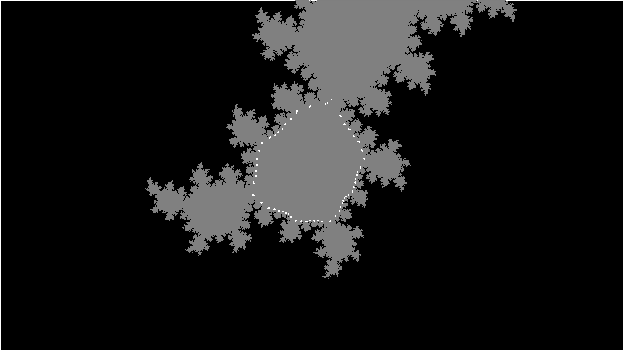
\includegraphics[width=0.8\textwidth]{../resources/ch-11/postcrit.png}
\caption{grey: a filled Julia set. White: the forward orbit of the critical point $-\lambda/2$, delineating the boundary of a Siegel disc
}}
\note{graphic is a screenshot of GLSL code that took five minutes to write. Make better ones.}
\end{figure}


\end{document}